%
% introduction.tex
%
% Copyright The SLCam Contributors.
%
% SLCam Documentation
%
% This work is licensed under the Creative Commons Attribution-ShareAlike 4.0
% International License. To view a copy of this license,
% visit http://creativecommons.org/licenses/by-sa/4.0/.
%

%
% \brief Introduction chapter.
%
% \author Gabriel Mariano Marcelino <gabriel.mm8@gmail.com>
%
% \version 0.3.0
%
% \date 2021/04/01
%

\chapter{Introduction} \label{ch:introduction}

The SLCam \nomenclature{\textbf{SLCam}}{\textit{SpaceLab Camera}} is a controller for a image sensor module designed to be used in nanosatellite missions. The main object is to take pictures of the Earth from space. It's the first project from SpaceLab using cameras in payloads.

\begin{figure}[!ht]
    \begin{center}
        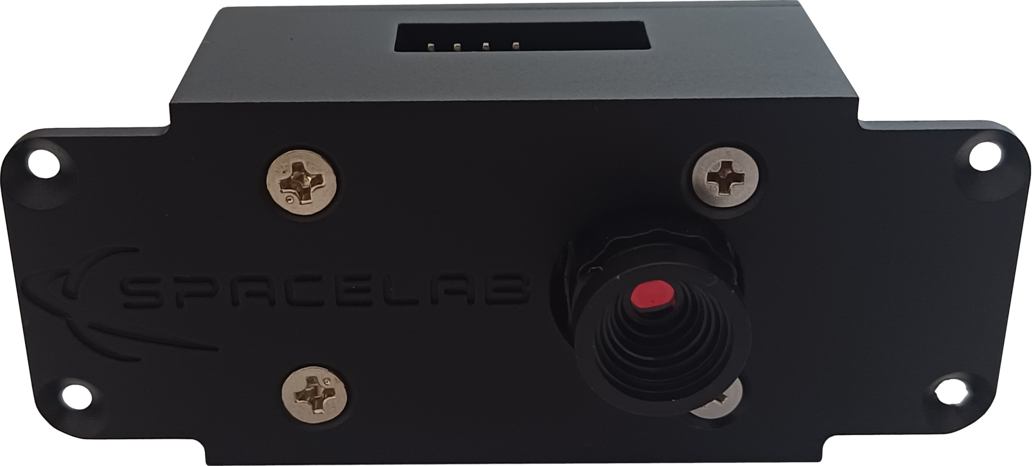
\includegraphics[width=0.7\textwidth]{figures/slcam-small.png}
        \caption{SLCam.}
        \label{fig:slcam-mounted}
    \end{center}
\end{figure}

\section{Product tree}

The product tree of the SLCam payload can be divided into five branches: hardware, firmware, mechanical, software and documentation. A diagram of the product tree is available in \autoref{fig:product-tree}.

\begin{figure}[!ht]
    \begin{center}
        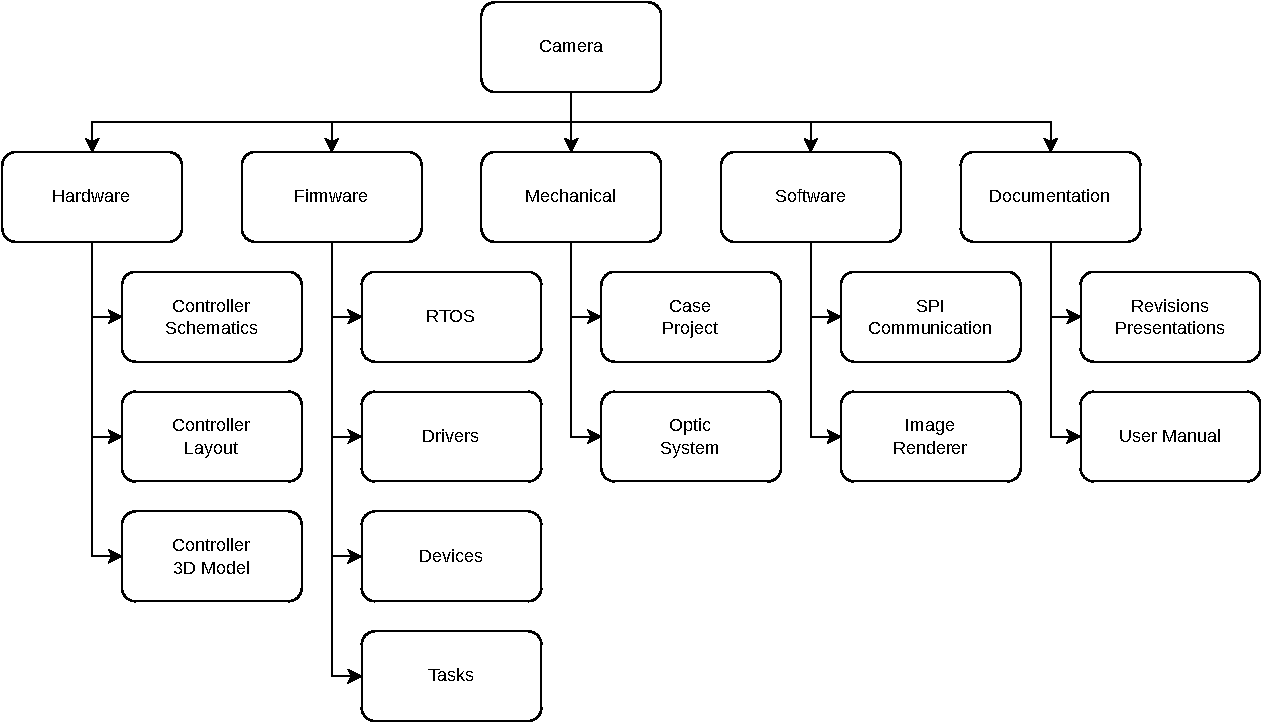
\includegraphics[width=\textwidth]{figures/product-tree.pdf}
        \caption{Product tree of the SLCam Payload.}
        \label{fig:product-tree}
    \end{center}
\end{figure}
